\documentclass[border=4pt]{standalone}
\usepackage{tikz}
\usetikzlibrary{decorations.pathmorphing,arrows.meta}
\begin{document}
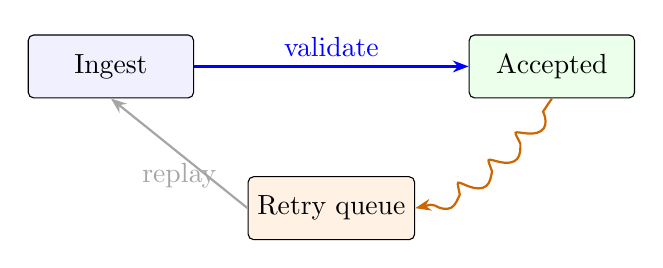
\begin{tikzpicture}[
  stage/.style={draw,rounded corners=2pt,minimum width=21mm,minimum height=8mm,fill=blue!6},
  route/.style={line width=.8pt,-{Stealth[length=2mm]}}
]
  \node[stage] (ingest) at (-2.8,0) {Ingest};
  \node[stage,fill=green!8] (accept) at (2.8,0) {Accepted};
  \node[stage,fill=orange!10] (retry) at (0,-1.8) {Retry queue};
  \draw[route,blue] (ingest) -- node[above]{validate} (accept);
  \draw[route,orange!80!black,decorate,
    decoration={coil,aspect=.35,segment length=5mm,amplitude=1.3mm,pre length=2mm,post length=2mm}]
    (accept.south) .. controls (2.1,-1.5) and (1.25,-1.8) .. (retry.east);
  \draw[route,gray!70] (retry.west) -- node[below]{replay} (ingest.south);
\end{tikzpicture}
\end{document}
